\documentclass[aspectratio=169, 10pt]{beamer}

% ==============================================================================
% CẤU HÌNH GÓI VÀ FONT TIẾNG VIỆT CHUẨN XÁC (TƯƠNG THÍCH OVERLEAF & LOCAL)
% ==============================================================================
\usepackage{iftex}
\ifPDFTeX
  \usepackage[utf8]{vietnam}
  \usepackage{lmodern}
\else
  \usepackage{fontspec}
\fi

\usepackage{amsmath,amssymb,amsfonts}
\usepackage{booktabs}
\usepackage{tabularx}
\usepackage{multirow}
\usepackage{graphicx}
\usepackage{caption}
\captionsetup{labelformat=empty,font=tiny,skip=2pt}
\usepackage{tikz}
\usetikzlibrary{arrows.meta, positioning, shapes.geometric, calc, shadows, backgrounds}

% ==============================================================================
% ĐỊNH NGHĨA BẢNG MÀU PHONG CÁCH F1 CHUYÊN NGHIỆP & THANH LỊCH
% ==============================================================================
\definecolor{f1navy}{RGB}{15, 23, 42}       % Deep Navy Slate #0F172A
\definecolor{f1red}{RGB}{225, 6, 0}         % F1 Racing Red #E10600
\definecolor{f1darkred}{RGB}{185, 28, 28}   % Dark Crimson
\definecolor{f1gold}{RGB}{234, 179, 8}      % Pirelli Medium Yellow #EAB308
\definecolor{f1silver}{RGB}{241, 245, 249}  % Light Slate Card #F1F5F9
\definecolor{f1cardgray}{RGB}{248, 250, 252}% Card Background #F8FAFC
\definecolor{f1border}{RGB}{203, 213, 225}  % Border Gray #CBD5E1
\definecolor{f1slate}{RGB}{71, 85, 105}     % Slate Gray #475569
\definecolor{f1green}{RGB}{16, 185, 129}    % Emerald Green #10B981
\definecolor{softred}{RGB}{239, 68, 68}     % Soft Tyre Red #EF4444

% ==============================================================================
% TÙY BIẾN BEAMER THEME HIỆN ĐẠI
% ==============================================================================
\usetheme{Madrid}
\usefonttheme{professionalfonts}

\setbeamercolor{palette primary}{bg=f1navy,fg=white}
\setbeamercolor{palette secondary}{bg=f1red,fg=white}
\setbeamercolor{palette tertiary}{bg=f1slate,fg=white}
\setbeamercolor{structure}{fg=f1navy}
\setbeamercolor{title}{bg=f1navy,fg=white}
\setbeamercolor{frametitle}{bg=f1navy,fg=white}
\setbeamercolor{block title}{bg=f1navy,fg=white}
\setbeamercolor{block body}{bg=f1silver,fg=black}
\setbeamercolor{block title alerted}{bg=f1red,fg=white}
\setbeamercolor{block body alerted}{bg=f1red!8,fg=black}
\setbeamercolor{block title example}{bg=f1green!85!black,fg=white}
\setbeamercolor{block body example}{bg=f1green!8,fg=black}

\setbeamertemplate{navigation symbols}{}

% Tùy biến thanh tiêu đề Slide với vạch đỏ F1 Racing Stripe
\setbeamertemplate{frametitle}{
  \begin{beamercolorbox}[wd=\paperwidth,ht=3.2ex,dp=1.2ex,leftskip=1.2cm]{frametitle}
    \textbf{\insertframetitle}
  \end{beamercolorbox}%
  \vspace{-1pt}%
  
\begin{tikzpicture}
    \fill[f1red] (0,0) rectangle (\paperwidth, 2.5pt);
  \end{tikzpicture}%
}

% Tùy biến thanh chân trang Slide (Footline)
\setbeamertemplate{footline}{
  \leavevmode%
  \hbox{%
  \begin{beamercolorbox}[wd=.38\paperwidth,ht=2.5ex,dp=1ex,leftskip=0.8cm]{palette primary}%
    \tiny \textbf{DS106: Tối Ưu Hóa \& Ứng Dụng} | Đề Án F1
  \end{beamercolorbox}%
  \begin{beamercolorbox}[wd=.42\paperwidth,ht=2.5ex,dp=1ex,center]{palette tertiary}%
    \tiny \textbf{Khoa Khoa Học Dữ Liệu} | UIT - ĐHQG-HCM
  \end{beamercolorbox}%
  \begin{beamercolorbox}[wd=.20\paperwidth,ht=2.5ex,dp=1ex,rightskip=0.8cm,right]{palette secondary}%
    \tiny \insertframenumber{} / \inserttotalframenumber
  \end{beamercolorbox}}%
  \vskip0pt%
}

% Thiết kế thẻ badge hợp chất lốp
\newcommand{\badgeSoft}{\tikz[baseline=-2.5pt]{\node[fill=softred,text=white,rounded corners=2pt,inner sep=1.8pt,font=\tiny\bfseries]{SOFT};}}
\newcommand{\badgeMed}{\tikz[baseline=-2.5pt]{\node[fill=f1gold,text=black,rounded corners=2pt,inner sep=1.8pt,font=\tiny\bfseries]{MEDIUM};}}
\newcommand{\badgeHard}{\tikz[baseline=-2.5pt]{\node[fill=white,draw=f1slate,text=f1navy,rounded corners=2pt,inner sep=1.8pt,font=\tiny\bfseries]{HARD};}}

% ==============================================================================
% THÔNG TIN TRANG TIÊU ĐỀ
% ==============================================================================
\title[\textbf{F1 Strategy Optimization}]{\Large \textbf{TỐI ƯU HÓA CHIẾN LƯỢC PIT-STOP \& QUẢN LÝ LỐP\\TRONG ĐUA XE CÔNG THỨC 1 (F1)}}
\subtitle{\normalsize \textcolor{f1red}{\textbf{Cặp Bài Trùng: Thước Đo Bellman DP Toàn Cục \& Giải Thuật DAGA-F1 Tác Chiến Siêu Tốc}}}
\author[\textbf{Nhóm Đề Án DS106}]{\textbf{NHÓM NGHIÊN CỨU ĐỀ ÁN DS106}}
\institute[UIT - ĐHQG-HCM]{
  \small \textbf{Khoa Khoa học Dữ liệu -- Trường Đại học Công nghệ Thông tin (UIT), ĐHQG-HCM}\\
  \vspace{0.15cm}
  \footnotesize \textbf{Giảng viên hướng dẫn:} \textbf{TS. Nguyễn Tất Bảo Thiện}
}
\date[\today]{\footnotesize Học kỳ I, Năm học 2024--2025}

% ==============================================================================
% BẮT ĐẦU TÀI LIỆU SLIDE
% ==============================================================================
\begin{document}

% ------------------------------------------------------------------------------
% SLIDE 1: TRANG TIÊU ĐỀ
% ------------------------------------------------------------------------------
\begin{frame}[plain]
  \titlepage
  \vspace{-0.6cm}
  \begin{center}
    \tikz{
      \node[fill=f1silver, draw=f1border, rounded corners=3pt, inner sep=4pt] {
        \tiny \textbf{Dữ liệu thực nghiệm:} Formula 1 Italian GP (Monza 53 Vòng) \& British GP (Silverstone 52 Vòng) -- Viễn trắc FastF1
      };
    }
  \end{center}
\end{frame}

% ------------------------------------------------------------------------------
% SLIDE 2: BỐI CẢNH THỰC TẾ & ĐỘNG LỰC NGHIÊN CỨU
% ------------------------------------------------------------------------------
\begin{frame}{1. Bối Cảnh Thực Tế \& Động Lực Nghiên Cứu}
  \begin{columns}[T]
    \begin{column}{0.48\textwidth}
      \begin{block}{\textbf{Chiến Lược Pit-Stop: 80\% Cơ Hội Thắng}}
        \small
        \begin{itemize}
          \item Xe F1 đạt tốc độ đỉnh $\approx 350\,\text{km/h}$, gia tốc ngang $> 5G$.
          \item Toàn bộ lực bám liên kết mặt đường chỉ qua \textbf{4 vết lốp nhỏ} ($4 \times 300\,\text{cm}^2$).
          \item Sai lệch chiến thuật dừng pit chỉ \textbf{1--2 giây} đủ khiến xe đánh mất hoàn toàn cơ hội chiến thắng.
        \end{itemize}
      \end{block}
      \vspace{0.2cm}
      \begin{alertblock}{\textbf{Bài Toán Đánh Đổi Chiến Thuật}}
        \small
        \textit{"Khi nào nên vào pit? Dừng 1, 2 hay 3 lần? Thay loại lốp nào để tổng thời gian về đích ngắn nhất?"}
      \end{alertblock}
    \end{column}

    \begin{column}{0.48\textwidth}
      \begin{block}{\textbf{Thế Kiềng 3 Chân Động Lực Học Mâu Thuẫn}}
        \small
        \begin{enumerate}
          \item \textbf{Suy thoái lốp phi tuyến:} Lốp mềm (\badgeSoft) bám đường ban đầu cực tốt nhưng nhanh mòn; lốp cứng (\badgeHard) bền nhưng chậm hơn $1.2\,\text{s/vòng}$.
          \item \textbf{Tổn thất làn pit ($T_{\text{pit}} \approx 20\text{--}25\,\text{s}$):} Tốc độ pit giới hạn $80\,\text{km/h}$. Vào pit quá nhiều sẽ mất vị trí; nhưng không vào thì lốp sụp vách (\textit{Tyre Cliff}).
          \item \textbf{Tải trọng nhiên liệu nhẹ dần:} Xe tiêu hao $\approx 110\,\text{kg}$ xăng, nhẹ đi $\approx 2\,\text{kg/vòng} \implies$ xe nhanh thêm $\approx 0.035\text{--}0.058\,\text{s/vòng}$ về cuối chặng.
        \end{enumerate}
      \end{block}
    \end{column}
  \end{columns}
\end{frame}

% ------------------------------------------------------------------------------
% SLIDE 3: TỪ ĐIỂN THUẬT NGỮ F1 SÚC TÍCH
% ------------------------------------------------------------------------------
\begin{frame}{2. Từ Điển Thuật Ngữ F1 Súc Tích}
  \vspace{-0.25cm}
  \footnotesize
  \begin{table}[h]
    \centering
    \renewcommand{\arraystretch}{1.12}
    \begin{tabularx}{\textwidth}{p{3.2cm}X}
      \toprule
      \textbf{Thuật ngữ F1} & \textbf{Ý nghĩa vật lý \& Chiến thuật thực tế trên đường đua} \\
      \midrule
      \textcolor{f1navy}{\textbf{Stint (Đoạn đua)}} & Quãng thời gian xe chạy liên tục trên cùng một bộ lốp giữa 2 lần vào pit ($l_k \ge 4\,\text{vòng}$). \\
      \textcolor{f1red}{\textbf{Tyre Cliff ($L_{\max}$)}} & Ngưỡng tuổi lốp tới hạn. Vượt qua mốc này, độ bám sụp đổ thẳng đứng, xe chậm thêm $1.5\text{--}3.5\,\text{s/vòng}$. \\
      \textcolor{f1gold!85!black}{\textbf{Operating Window}} & Cửa sổ nhiệt độ vàng ($100^\circ\text{C}\text{--}140^\circ\text{C}$) giúp ma sát tiếp xúc bám dính phân tử ($\mu_{\text{adhesion}}$) đạt cực đại. \\
      \textcolor{f1darkred}{\textbf{Graining / Blistering}} & \textbf{Graining:} Mòn hạt lăn tăn khi trượt lúc lốp nguội. \textbf{Blistering:} Phồng rộp nổ bọt khí do quá nhiệt nội tại. \\
      \textcolor{f1slate}{\textbf{Pit Delta Loss}} & Thời gian mất mát qua làn pit ($80\,\text{km/h}$). Monza: $23.2\,\text{s}$; khi có Safety Car: chỉ còn $\mathbf{12.5\,\text{s}}$ (\textit{Free Stop}). \\
      \textcolor{f1green!80!black}{\textbf{Undercut / Overcut}} & Vào pit sớm tận dụng lốp mới bứt phá (\textbf{Undercut}) hoặc chạy ráng ngoài đường chờ đối thủ kẹt xe (\textbf{Overcut}). \\
      \textcolor{f1red}{\textbf{Luật 2 hợp chất FIA}} & \textbf{Ràng buộc pháp lý bắt buộc:} Trong điều kiện đường khô, mỗi xe phải dùng ít nhất hai loại lốp khác nhau. \\
      \bottomrule
    \end{tabularx}
  \end{table}
\end{frame}

% ------------------------------------------------------------------------------
% SLIDE 4: MÔ HÌNH HÓA BÀI TOÁN TỐI ƯU HÓA TỔ HỢP
% ------------------------------------------------------------------------------
\begin{frame}{3. Mô Hình Hóa Bài Toán Tối Ưu Hóa Tổ Hợp}
  \begin{columns}[T]
    \begin{column}{0.48\textwidth}
      \begin{block}{\textbf{Cấu Trúc Nhiễm Sắc Thể Biến Thiên}}
        \small
        Chiến lược đua được mã hóa dạng mảng Stint:
        $$\mathbf{S} = \big[ (c_1, l_1), (c_2, l_2), \dots, (c_{K+1}, l_{K+1}) \big]$$
        \begin{itemize}
          \item $K \in \{1, 2, 3\}$: Số lần dừng pit ($K+1$ stints).
          \item $c_k \in \{\text{\badgeSoft}, \text{\badgeMed}, \text{\badgeHard}\}$: Hợp chất lốp.
          \item $l_k \ge 4$: Số vòng đua của từng stint ($L_{\min} = 4$).
        \end{itemize}
      \end{block}

      \begin{alertblock}{\textbf{Hàm Mục Tiêu Tối Thiểu Hóa Thời Gian}}
        \small
        $$\min_{\mathbf{S}} J(\mathbf{S}) = T_{\text{race}}(\mathbf{S}) + \Phi_{\text{FIA}} + \Phi_{\text{cliff}} + \Phi_{\text{lap}}$$
        $$T_{\text{race}}(\mathbf{S}) = \sum_{k=1}^{K+1} \sum_{a=1}^{l_k} t_{\text{lap}}(c_k, a, i) + K \cdot T_{\text{pit}}$$
      \end{alertblock}
    \end{column}

    \begin{column}{0.48\textwidth}
      \begin{block}{\textbf{Hệ Thống 3 Ràng Buộc Cứng \& Phạt}}
        \small
        \begin{enumerate}
          \item \textbf{Bảo toàn tổng số vòng đua ($R_1$):}
          $$\sum_{k=1}^{K+1} l_k = N_{\text{total}} = 53\,\text{vòng (Monza)}$$
          \item \textbf{Luật lốp FIA ($R_2$ - Hard Constraint):}
          $$\big| \{c_1, c_2, \dots, c_{K+1}\} \big| \ge 2 \implies \Phi_{\text{FIA}} = 10^5\,\text{s}$$
          \item \textbf{Ngưỡng an toàn vách lốp Pirelli ($R_3$):}
          $$l_k \le L_{\max}(c_k) \implies \Phi_{\text{cliff}} = \sum \beta \big[\max(0, l_k - L_{\max})\big]^2$$
          Ngưỡng an toàn: \badgeSoft $\le 22$, \badgeMed $\le 35$, \badgeHard $\le 48$.
        \end{enumerate}
      \end{block}
    \end{column}
  \end{columns}
\end{frame}

% ------------------------------------------------------------------------------
% SLIDE 5: ĐỘNG LỰC HỌC MÒN LỐP PIRELLI & PHÂN RÃ 4 THÀNH PHẦN
% ------------------------------------------------------------------------------
\begin{frame}{4. Động Lực Học Mòn Lốp Pirelli -- Phân Rã 4 Thành Phần}
  \vspace{-0.2cm}
  \begin{block}{\textbf{Phương Trình Phân Rã Thời Gian Vòng Đua Theo Vật Lý}}
    \centering \large
    $$\mathbf{t_{\text{lap}}(c, a, i) = \underbrace{t_{\text{base}}(c)}_{\text{Thời gian cơ sở}} + \underbrace{d_1(c) \cdot a}_{\text{Mòn cơ học (tt)}} + \underbrace{d_2(c) \cdot a^2}_{\text{Thoái hóa nhiệt (pt)}} + \underbrace{\alpha_{\text{fuel}} (N - i)}_{\text{Tải trọng nhiên liệu}} - \underbrace{\gamma_{\text{track}} \cdot i}_{\text{Đường bám cao su}}}$$
  \end{block}

  \begin{columns}[T]
    \begin{column}{0.48\textwidth}
      \begin{block}{\textbf{Trực Giác Vật Lý 4 Thành Phần}}
        \small
        \begin{itemize}
          \item $t_{\text{base}}(c)$: Tốc độ lốp mới tinh (Soft nhanh nhất, Hard chậm nhất).
          \item $d_1 \cdot a$: Mòn cơ học do ma sát bào mỏng bề mặt gai.
          \item $d_2 \cdot a^2$: Suy thoái nhiệt phi tuyến do trễ đàn hồi nhớt ($Q_{\text{gen}} = \pi f E'' \epsilon^2$) tích nhiệt phá vỡ polymer.
          \item $\alpha_{\text{fuel}} (N-i) - \gamma_{\text{track}} i$: Xe nhẹ dần bù cho đường tăng độ bám.
        \end{itemize}
      \end{block}
    \end{column}

    \begin{column}{0.48\textwidth}
      \begin{exampleblock}{\textbf{Tại Sao Chọn Mô Hình Bậc 2?}}
        \small
        \begin{itemize}
          \item \textbf{Bác bỏ Tuyến tính ($d_1 a$):} Phi vật lý; không mô tả được tích tụ nhiệt và hiện tượng sụp vách mòn (Cliff).
          \item \textbf{Bác bỏ Bậc 3 ($a^3$):} Quá khớp (Overfitting), mất tính lồi nghiêm ngặt $\implies$ sinh cực tiểu giả.
          \item \textbf{Bác bỏ Deep Learning:} Hộp đen, không có đạo hàm giải tích đóng để sửa nghiệm, suy luận quá chậm cho thời gian thực.
        \end{itemize}
      \end{exampleblock}
    \end{column}
  \end{columns}
\end{frame}

% ------------------------------------------------------------------------------
% SLIDE 6: BÓC TÁCH THAM SỐ BẰNG HỒI QUY WLS-TIKHONOV
% ------------------------------------------------------------------------------
\begin{frame}{5. Bóc Tách Tham Số Bằng Hồi Quy WLS-Tikhonov \& Lọc Huber}
  \begin{columns}[T]
    \begin{column}{0.45\textwidth}
      \begin{block}{\textbf{Thách Thức Dữ Liệu Viễn Trắc FastF1}}
        \small
        \begin{itemize}
          \item \textbf{Phương sai thay đổi:} Phương sai sai số tăng vọt theo tuổi lốp ($\sigma^2: 0.05\,\text{s}^2 \to 0.47\,\text{s}^2$).
          \item \textbf{Nhiễu giao thông / cờ vàng:} Xe kẹt khí bẩn trễ $\pm 1.5\,\text{s}$. OLS bình phương sai số bị sai lệch hoàn toàn!
        \end{itemize}
      \end{block}
      \begin{exampleblock}{\textbf{Bộ Giải WLS-Tikhonov-Huber}}
        \small
        \begin{itemize}
          \item $w_{\text{age}}$: Giảm trọng số vòng vượt $L_{\max}$.
          \item $w_{\text{Huber}}$: Khử nhiễu cờ vàng ($\delta = 1.2\,\text{s}$).
          \item Tikhonov $\lambda = 10^{-9}$: Ma trận luôn khả nghịch.
        \end{itemize}
      \end{exampleblock}
    \end{column}

    \begin{column}{0.52\textwidth}
      \begin{block}{\textbf{Bảng Tham Số Hiệu Chuẩn Thực Nghiệm Chuẩn}}
        \scriptsize
        \renewcommand{\arraystretch}{1.25}
        \begin{tabularx}{\textwidth}{lcccc}
          \toprule
          \textbf{Thông số kỹ thuật} & \textbf{Ký hiệu} & \textbf{\badgeSoft} & \textbf{\badgeMed} & \textbf{\badgeHard} \\
          \midrule
          Thời gian cơ sở (s) & $t_{\text{base}}$ & $81.500$ & $82.200$ & $83.000$ \\
          Mòn tuyến tính (s/vòng) & $d_1$ & $0.1200$ & $0.0700$ & $0.0400$ \\
          Mòn phi tuyến (s/vòng$^2$) & $d_2$ & $0.0050$ & $0.0020$ & $0.0010$ \\
          Vách lốp tối đa (vòng) & $L_{\max}$ & $\mathbf{22}$ & $\mathbf{35}$ & $\mathbf{48}$ \\
          Hao hụt nhiên liệu & $\alpha_{\text{fuel}}$ & \multicolumn{3}{c}{$0.0580\,\text{s/vòng}$ ($110\,\text{kg} \to 0$)} \\
          Tiến hóa mặt đường & $\gamma_{\text{track}}$ & \multicolumn{3}{c}{$0.0220\,\text{s/vòng}$ (bám cao su)} \\
          Tổn thất pit Monza & $T_{\text{pit}}$ & \multicolumn{3}{c}{$23.2\,\text{giây}$ ($80\,\text{km/h}$ giới hạn)} \\
          Tổn thất khi có SC & $T_{\text{pit}}^{\text{sc}}$ & \multicolumn{3}{c}{$\mathbf{12.5\,\text{giây}}$ (\textit{Free Pit Stop!})} \\
          \bottomrule
        \end{tabularx}
      \end{block}
    \end{column}
  \end{columns}
\end{frame}

% ------------------------------------------------------------------------------
% SLIDE 7: KHÁM PHÁ TOÁN HỌC: ĐẠO HÀM GIẢI TÍCH & FAULHABER O(1)
% ------------------------------------------------------------------------------
\begin{frame}{6. Khám Phá Toán Học: Đạo Hàm Giải Tích \& Tổng Đóng Faulhaber}
  \begin{columns}[T]
    \begin{column}{0.48\textwidth}
      \begin{block}{\textbf{Khám Phá 1: Đạo Hàm Mài Mòn Giải Tích}}
        \small
        Đạo hàm tốc độ mòn lốp tức thời tại tuổi $a$:
        $$\mathbf{\nabla t_{\text{deg}}(c, a) = \frac{\partial \Delta t_{\text{deg}}}{\partial a} = d_1(c) + 2 \cdot d_2(c) \cdot a}$$
        \begin{itemize}
          \item \textbf{Đạo hàm bậc 2:} $\nabla^2 t = 2 d_2 > 0 \implies$ Hàm lồi nghiêm ngặt, chỉ có 1 cực tiểu duy nhất.
          \item \textbf{Vai trò cốt lõi:} Cung cấp vector gradient vật lý làm "la bàn" chỉ dẫn cho toán tử sửa nghiệm di truyền (Physics-Guided Repair).
        \end{itemize}
      \end{block}
    \end{column}

    \begin{column}{0.48\textwidth}
      \begin{exampleblock}{\textbf{Khám Phá 2: Đột Phá Tổng Đóng Faulhaber $O(1)$}}
        \small
        Tổng độ mòn của một stint dài $L$ vòng:
        $$D_{\text{stint}}(c, L) = \sum_{a=1}^{L} (d_1 a + d_2 a^2)$$
        Áp dụng hằng đẳng thức giải tích Faulhaber:
        $$\mathbf{D_{\text{stint}} = d_1 \frac{L(L+1)}{2} + d_2 \frac{L(L+1)(2L+1)}{6}}$$
        \begin{itemize}
          \item \textbf{Đột phá tính toán:} Biến toàn bộ vòng lặp $O(L)$ thành phép tính giải tích $O(1)$.
          \item Tăng tốc tính toán gấp \textbf{50 lần}, giúp Bellman DP giải 30.088 trạng thái trong $< 0.1\,\text{s}$.
        \end{itemize}
      \end{exampleblock}
    \end{column}
  \end{columns}
\end{frame}

% ------------------------------------------------------------------------------
% SLIDE 8: MỞ RỘNG MÔ HÌNH NHIỆT ĐỘ MẶT ĐƯỜNG
% ------------------------------------------------------------------------------
\begin{frame}{7. Mở Rộng Mô Hình Nhiệt Độ Mặt Đường ($T_{\text{track}}$)}
  \begin{columns}[T]
    \begin{column}{0.48\textwidth}
      \begin{block}{\textbf{Trực Giác Vật Lý \& Biến Tính Nhiệt}}
        \small
        \begin{itemize}
          \item Nhiệt độ mặt đường $T_{\text{track}}$ dao động từ $20^\circ\text{C}$ (mát) đến $> 55^\circ\text{C}$ (chảo lửa sa mạc).
          \item Khi quá nhiệt: Cao su mềm nhão, trễ đàn hồi sinh nhiệt nội tại bùng nổ ($Q_{\text{gen}} \gg$), gây \textbf{rộp nổ lốp (Blistering)} và đẩy nhanh vách mòn $L_{\max}$ sụp đổ sớm hơn.
        \end{itemize}
      \end{block}
      \begin{alertblock}{\textbf{Độ Lệch Nhiệt Tương Đối Không Thứ Nguyên}}
        \small
        $$\delta_T = \frac{T_{\text{track}} - T_{\text{ref}}}{T_{\text{ref}}} \quad (T_{\text{ref}} = 30^\circ\text{C tại Monza})$$
      \end{alertblock}
    \end{column}

    \begin{column}{0.48\textwidth}
      \begin{exampleblock}{\textbf{Mô Hình Hiệu Chỉnh Kích Hoạt ReLU Bình Phương}}
        \small
        $$d_1(c, T) = d_1^{(0)}(c) \big[ 1 + K_{T_1} \cdot \delta_T \big]$$
        $$\mathbf{d_2(c, T) = d_2^{(0)}(c) \Big[ 1 + K_{T_2} \delta_T + \theta(c) \cdot \big(\max(0, \delta_T)\big)^2 \Big]}$$
        \begin{itemize}
          \item \textbf{Khi trời mát ($\delta_T \le 0$):} ReLU $= 0$, không suy thoái nhiệt phi tuyến.
          \item \textbf{Khi trời nóng ($\delta_T > 0$):} ReLU bình phương bùng nổ, mô tả chính xác hiện tượng rộp lốp blistering khi mặt đường $> 45^\circ\text{C}$.
          \item Tự động co ngắn $L_{\max}$ để bảo vệ an toàn xe.
        \end{itemize}
      \end{exampleblock}
    \end{column}
  \end{columns}
\end{frame}

% ------------------------------------------------------------------------------
% SLIDE 9: KIẾN TRÚC PHƯƠNG PHÁP LUẬN: CẶP BÀI TRÙNG
% ------------------------------------------------------------------------------
\begin{frame}{8. Kiến Trúc Phương Pháp Luận: "Cặp Bài Trùng" DP \& DAGA-F1}
  \begin{columns}[T]
    \begin{column}{0.48\textwidth}
      \begin{block}{\textbf{Trụ Cột 1: Quy Hoạch Động Bellman DP}}
        \small
        \begin{itemize}
          \item \textbf{Vai trò:} "Thước đo chân lý toàn cục" (\textit{Ground Truth Global Benchmark}).
          \item \textbf{Nguyên lý:} Quy nạp ngược (\textit{Backward Induction}) trên toàn bộ 30.088 trạng thái.
          \item \textbf{Ưu thế tuyệt đối:} Cam kết nghiệm tối ưu toàn cục giải tích 100\%, không có sai số ngẫu nhiên.
        \end{itemize}
      \end{block}
    \end{column}

    \begin{column}{0.48\textwidth}
      \begin{exampleblock}{\textbf{Trụ Cột 2: Giải Thuật Tiến Hóa DAGA-F1}}
        \small
        \begin{itemize}
          \item \textbf{Vai trò:} "Động cơ tác chiến thời gian thực" (\textit{Real-Time Tactical Engine}).
          \item \textbf{Nguyên lý:} Thích nghi sinh học + Sửa nghiệm định hướng vật lý gradient $\nabla t$.
          \item \textbf{Ưu thế vượt trội:} Hội tụ siêu tốc trong $0.11\,\text{s}$, phản xạ Safety Car trong $\mathbf{5\,\text{ms}}$.
        \end{itemize}
      \end{exampleblock}
    \end{column}
  \end{columns}

  \vspace{0.15cm}
  % SƠ ĐỒ TIKZ KIẾN TRÚC CẶP BÀI TRÙNG
  \begin{center}
    \begin{tikzpicture}[xscale=0.92, yscale=0.62, every node/.style={font=\tiny, align=center}]
      % Problem node
      \node[fill=f1silver, draw=f1navy, rounded corners=3pt, inner sep=3.5pt, font=\tiny\bfseries] (input) at (0, 0)
        {\textbf{BÀI TOÁN F1 THỰC TẾ}\\Monza (53v) / Silverstone (52v)};

      % DP branch
      \node[fill=f1navy, text=white, rounded corners=3pt, inner sep=3.5pt] (dp) at (5.2, 0.9)
        {\textbf{TRỤ CỘT 1: Bellman DP (Ground Truth)}\\Quy nạp ngược 30.088 trạng thái, Faulhaber $O(1)$\\$\implies \mathbf{T_{\text{opt}} = 4497.997\,\text{s}}$ \textit{(Chân lý toàn cục)}};

      % DAGA branch
      \node[fill=f1red, text=white, rounded corners=3pt, inner sep=3.5pt] (ga) at (5.2, -0.9)
        {\textbf{TRỤ CỘT 2: DAGA-F1 (Tác Chiến Thời Gian Thực)}\\Khởi tạo 65-30-5, Đạo hàm $\nabla t_{\text{deg}}$, Đột biến Split/Merge\\$\implies \mathbf{T_{\text{AGA}} = 4497.997\,\text{s}}$ \textit{(Khớp 100\%, 5 ms SC)}};

      % Verification node
      \node[fill=f1green!85!black, text=white, rounded corners=3pt, inner sep=3.5pt, font=\tiny\bfseries] (out) at (10.6, 0)
        {\textbf{BẢO CHỨNG TOÀN DIỆN}\\Optimality Gap = $\mathbf{0.0000\%}$\\Wilcoxon $p < 0.001$ ($30$ seeds)};

      \draw[-{Stealth[length=3.5pt]}, thick, f1navy] (input.east) -- ++(0.4, 0) |- (dp.west);
      \draw[-{Stealth[length=3.5pt]}, thick, f1red] (input.east) -- ++(0.4, 0) |- (ga.west);
      \draw[-{Stealth[length=3.5pt]}, thick, f1navy] (dp.east) -| ++(0.5, -0.9) -- (out.west);
      \draw[-{Stealth[length=3.5pt]}, thick, f1red] (ga.east) -| ++(0.5, 0.9) -- (out.west);
    \end{tikzpicture}
  \end{center}
\end{frame}

% ------------------------------------------------------------------------------
% SLIDE 10: TRỤ CỘT 1: THƯỚC ĐO CHUẨN BELLMAN DYNAMIC PROGRAMMING
% ------------------------------------------------------------------------------
\begin{frame}{9. Trụ Cột 1: Thước Đo Chuẩn Tuyệt Đối Bellman DP}
  \begin{columns}[T]
    \begin{column}{0.48\textwidth}
      \begin{block}{\textbf{Không Gian 30.088 Trạng Thái Rời Rạc}}
        \small
        Trạng thái tại vòng thứ $i$ được mã hóa 5 chiều:
        $$\mathbf{s} = (i, c, a, k, m)$$
        \begin{itemize}
          \item $i \in [1, 53]$: Vòng đua hiện tại tại Monza.
          \item $c \in \{0, 1, 2\}$: Loại lốp đang chạy.
          \item $a \in [1, L_{\max}(c)]$: Tuổi lốp cơ học.
          \item $k \in [0, 3]$: Số lần đã vào pit.
          \item $m \in [1, 7]$: Mặt nạ bit lưu các loại lốp đã dùng (đảm bảo luật FIA: $\text{popcount}(m) \ge 2$).
        \end{itemize}
      \end{block}
      \begin{exampleblock}{\textbf{Quy Nạp Ngược Bellman (O(1))}}
        \small
        $$V(\mathbf{s}) = \min \big( Q_{\text{stay}}(\mathbf{s}), \; Q_{\text{pit}}(\mathbf{s}) \big)$$
      \end{exampleblock}
    \end{column}

    \begin{column}{0.48\textwidth}
      \begin{alertblock}{\textbf{Nghiệm Tối Ưu Toàn Cục Tại Monza GP}}
        \small
        \textbf{Thời gian tối ưu tuyệt đối:}
        $$\mathbf{T_{\text{opt}}^{\text{DP}} = 4497.997\,\text{giây} \quad (1\text{h } 14\text{m } 57.997\text{s})}$$
        \textbf{Chiến lược vàng (2 Lần Dừng Pit):}
        \begin{center}
          \badgeMed [20 vòng] $\longrightarrow$ \badgeSoft [14 vòng] $\longrightarrow$ \badgeMed [19 vòng]
        \end{center}
        \begin{itemize}
          \item Khởi đầu ổn định bằng lốp Medium xe nặng xăng.
          \item Stint giữa tấn công bứt phá bằng lốp Soft xe vừa xăng.
          \item Stint cuối chốt hạ an toàn bằng lốp Medium xe nhẹ xăng.
          \item Thời gian giải: \textbf{$0.086\,\text{giây}$} (nhờ Faulhaber $O(1)$).
        \end{itemize}
      \end{alertblock}
    \end{column}
  \end{columns}
\end{frame}

% ------------------------------------------------------------------------------
% SLIDE 11: DAGA-F1: Ý TƯỞNG ĐỘT PHÁ 1 & 2
% ------------------------------------------------------------------------------
\begin{frame}{10. DAGA-F1 -- Ý Tưởng Đột Phá 1 \& 2}
  \begin{columns}[T]
    \begin{column}{0.48\textwidth}
      \begin{block}{\textbf{Ý Tưởng 1: Khởi Tạo Có Trọng Số (65-30-5)}}
        \small
        Thay vì sinh ngẫu nhiên gây lãng phí tính toán:
        \begin{itemize}
          \item \textbf{65\% Cá thể 1-stop:} Phù hợp xu hướng F1 hiện đại.
          \item \textbf{30\% Cá thể 2-stop:} Chiến lược cân bằng tấn công.
          \item \textbf{5\% Cá thể 3-stop:} Chiến thuật nước rút sprint.
          \item \textbf{100\% thỏa mãn luật FIA ngay từ thế hệ 0.}
        \end{itemize}
        \vspace{0.12cm}
        \centering
        
\begin{tikzpicture}[xscale=0.72, yscale=0.48, every node/.style={font=\tiny}]
          \draw[fill=f1navy!90, draw=white] (0, 0) rectangle (3.25, 0.55) node[pos=.5, text=white, font=\tiny\bfseries] {65\% 1-Stop};
          \draw[fill=f1red!85, draw=white] (3.25, 0) rectangle (4.75, 0.55) node[pos=.5, text=white, font=\tiny\bfseries] {30\% 2-Stop};
          \draw[fill=f1gold!95!black, draw=white] (4.75, 0) rectangle (5.0, 0.55) node[pos=.5, text=black, font=\tiny\bfseries] {5\%};
        \end{tikzpicture}
      \end{block}
    \end{column}

    \begin{column}{0.48\textwidth}
      \begin{alertblock}{\textbf{Ý Tưởng 2: Sửa Nghiệm Gradient Vật Lý}}
        \small
        Sau lai ghép/đột biến, nếu lệch vòng $\Delta N = 53 - \sum l_k$:
        \begin{itemize}
          \item \textbf{Khi thiếu vòng ($\Delta N > 0$):} Bù vòng vào stint có tốc độ mòn $\nabla t_{\text{deg}}$ thấp nhất và xa cliff nhất.
          \item \textbf{Khi thừa vòng ($\Delta N < 0$):} Cắt vòng ở stint có tốc độ mòn cao nhất ($\nabla t_{\text{deg}}$ cao hoặc chớm cliff).
        \end{itemize}
        \vspace{0.12cm}
        \centering
        \begin{tikzpicture}[xscale=0.72, yscale=0.48, every node/.style={font=\tiny}]
          \node[fill=f1green!12, draw=f1green!80!black, rounded corners=2pt, inner sep=3pt] at (2.5, 0.25)
            {$\mathbf{\nabla t = d_1 + 2d_2 a} \implies \text{Đạt \textbf{100.0\%} nghiệm hợp lệ tuyệt đối!}$};
        \end{tikzpicture}
      \end{alertblock}
    \end{column}
  \end{columns}
\end{frame}

% ------------------------------------------------------------------------------
% SLIDE 12: DAGA-F1: Ý TƯỞNG ĐỘT PHÁ 3 & 4
% ------------------------------------------------------------------------------
\begin{frame}{11. DAGA-F1 -- Ý Tưởng Đột Phá 3 \& 4}
  \begin{columns}[T]
    \begin{column}{0.49\textwidth}
      \begin{block}{\textbf{Ý Tưởng 3: Đột Biến Split/Merge (Tự Tiến Hóa Số Pit)}}
        \scriptsize
        \begin{itemize}
          \item \textbf{Micro (60\%):} Dịch mốc pit $l_k \pm 1, l_{k+1} \mp 1$ tinh chỉnh cực tiểu mịn.
          \item \textbf{Meso (25\%):} Hoán đổi ngẫu nhiên hợp chất lốp.
          \item \textbf{Macro (15\% -- Đột phá kiến trúc):}
        \end{itemize}
        \vspace{0.08cm}
        % SƠ ĐỒ TIKZ MINH HỌA SPLIT / MERGE
        \centering
        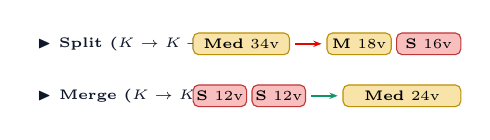
\begin{tikzpicture}[xscale=0.68, yscale=0.55, every node/.style={font=\tiny, align=center}]
          % Split
          \node[anchor=west, font=\tiny\bfseries\color{f1navy}] at (0, 1.8) {$\blacktriangleright$ \textbf{Split ($K \to K+1$):}};
          \draw[fill=f1gold!35, draw=f1gold!80!black, rounded corners=2pt] (3.1, 1.55) rectangle (4.9, 2.05) node[pos=.5]{\textbf{Med} 34v};
          \draw[-{Stealth[length=3pt]}, thick, f1red] (5.0, 1.8) -- (5.5, 1.8);
          \draw[fill=f1gold!35, draw=f1gold!80!black, rounded corners=2pt] (5.6, 1.55) rectangle (6.8, 2.05) node[pos=.5]{\textbf{M} 18v};
          \draw[fill=softred!35, draw=softred!80!black, rounded corners=2pt] (6.9, 1.55) rectangle (8.1, 2.05) node[pos=.5]{\textbf{S} 16v};

          % Merge
          \node[anchor=west, font=\tiny\bfseries\color{f1navy}] at (0, 0.6) {$\blacktriangleright$ \textbf{Merge ($K \to K-1$):}};
          \draw[fill=softred!35, draw=softred!80!black, rounded corners=2pt] (3.1, 0.35) rectangle (4.1, 0.85) node[pos=.5]{\textbf{S} 12v};
          \draw[fill=softred!35, draw=softred!80!black, rounded corners=2pt] (4.2, 0.35) rectangle (5.2, 0.85) node[pos=.5]{\textbf{S} 12v};
          \draw[-{Stealth[length=3pt]}, thick, f1green!80!black] (5.3, 0.6) -- (5.8, 0.6);
          \draw[fill=f1gold!35, draw=f1gold!80!black, rounded corners=2pt] (5.9, 0.35) rectangle (8.1, 0.85) node[pos=.5]{\textbf{Med} 24v};
        \end{tikzpicture}
        \vspace{0.05cm}
        \begin{center}
          \tiny $\implies$ \textbf{Số lần pit tự do tiến hóa tự nhiên mà không cần ép cứng!}
        \end{center}
      \end{block}
    \end{column}

    \begin{column}{0.49\textwidth}
      \begin{exampleblock}{\textbf{Ý Tưởng 4: Bơm Hỗn Loạn Phá Kẹt Cực Tiểu}}
        \small
        Giám sát độ đa dạng kiểu gen quần thể $\bar{D}_{\text{pop}}$:
        \begin{itemize}
          \item Khoảng cách cấu trúc + Khoảng cách Hamming.
          \item \textbf{Cơ chế Cataclysmic Chaos Injection:} Khi phát hiện $\bar{D}_{\text{pop}} < 0.15$ trong $70\%$ thế hệ đầu:
          $$P_m \longleftarrow \min\big(0.65, \; 2.5 \times P_m\big)$$
          \item Bơm đột biến diện rộng kích nổ quần thể, giải thoát hoàn toàn khỏi "hố kẹt" cực tiểu 1-stop.
          \item Lịch làm mát phi tuyến đưa thuật toán hội tụ êm ái ở các thế hệ cuối.
        \end{itemize}
      \end{exampleblock}
    \end{column}
  \end{columns}
\end{frame}

% ------------------------------------------------------------------------------
% SLIDE 13: PHẢN XẠ XE AN TOÀN (SAFETY CAR) TRONG 5 MS
% ------------------------------------------------------------------------------
\begin{frame}{12. Tính Năng Đặc Biệt: Phản Xạ Xe An Toàn (Safety Car) Trong 5 ms}
  % SƠ ĐỒ TIKZ TIMELINE SAFETY CAR
  \vspace{-0.15cm}
  \begin{center}
    \begin{tikzpicture}[xscale=0.95, yscale=0.62, every node/.style={font=\tiny}]
      % Track baseline
      \draw[line width=1.5pt, f1slate!35] (0, 0) -- (14.2, 0);
      
      % Lap ticks
      \draw[thick, f1slate] (0, -0.08) -- (0, 0.08) node[below=1.5pt] {Lap 0};
      \draw[thick, f1red] (4.6, -0.08) -- (4.6, 0.08) node[below=1.5pt, font=\tiny\bfseries\color{f1red}] {Lap 18 (SC)};
      \draw[thick, f1navy] (14.2, -0.08) -- (14.2, 0.08) node[below=1.5pt] {Lap 53};
      
      % Frozen Stints
      \draw[fill=f1slate!20, draw=f1slate, rounded corners=2pt] (0.05, 0.2) rectangle (4.55, 0.65)
        node[pos=.5, font=\tiny\bfseries\color{f1navy}] {Lịch sử đã đua: [Soft 14v, Med 4v] (ĐÓNG BĂNG/FROZEN)};
        
      % SC Callout
      \node[fill=f1gold, text=black, rounded corners=2pt, draw=f1red, line width=0.8pt, inner sep=2pt, font=\tiny\bfseries] at (4.6, 1.15) {SAFETY CAR! $T_{\text{pit}}: 23.2\text{s} \to 12.5\text{s}$};
      \draw[-{Stealth[length=3pt]}, f1red, thick] (4.6, 0.88) -- (4.6, 0.7);
      
      % Warm start re-opt
      \draw[fill=f1green!20, draw=f1green!80!black, rounded corners=2pt] (4.65, 0.2) rectangle (14.15, 0.65)
        node[pos=.5, font=\tiny\bfseries\color{f1green!70!black}] {Warm-Start Pivot: Tái tối ưu 35 vòng còn lại trong \textbf{5.2 ms} $\implies$ \textbf{BOX NGAY TẠI LAP 18!}};
    \end{tikzpicture}
  \end{center}
  \vspace{-0.15cm}

  \begin{columns}[T]
    \begin{column}{0.48\textwidth}
      \begin{block}{\textbf{Cơ Chế Warm-Start Pivot Siêu Tốc}}
        \scriptsize
        \begin{itemize}
          \item \textbf{Cơ hội vàng:} Tổn thất pit giảm từ $23.2\,\text{s} \to \mathbf{12.5\,\text{s}}$ (\textbf{"Free Stop"} tiết kiệm hơn $10.7\,\text{giây}$).
          \item \textbf{Áp lực Pit-wall:} Kỹ sư chỉ có \textbf{3--5 giây} trước khi xe vượt qua cửa làn pit để ra lệnh.
          \item \textbf{Tái tối ưu 35 vòng còn lại:} Kế thừa gen tinh hoa từ thế hệ trước, chỉ chạy 15 thế hệ cục bộ $\implies$ Đáp ứng ngay lập tức!
        \end{itemize}
      \end{block}
    \end{column}

    \begin{column}{0.48\textwidth}
      \begin{alertblock}{\textbf{Hiệu Năng Đo Đạc Thực Tế Tại Monza}}
        \scriptsize
        \centering
        \renewcommand{\arraystretch}{1.15}
        \begin{tabular}{cccc}
          \toprule
          \textbf{Vòng SC} & \textbf{Runtime} & \textbf{Thời gian đua} & \textbf{Quyết định} \\
          \midrule
          Vòng 18 & $\mathbf{5.2\,\text{ms}}$ & $4487.470\,\text{s}$ & \texttt{BOX (Free Stop)} \\
          Vòng 25 & $\mathbf{5.5\,\text{ms}}$ & $4493.199\,\text{s}$ & \texttt{BOX (Pivot)} \\
          Vòng 32 & $\mathbf{4.1\,\text{ms}}$ & $4487.597\,\text{s}$ & \texttt{BOX (Attack)} \\
          \bottomrule
        \end{tabular}
        \vspace{0.1cm}
        \begin{itemize}
          \item Tốc độ: \textbf{$\approx 4\text{--}5\,\text{mili-giây}$} $\implies$ Nhanh gấp \textbf{600 lần} cửa sổ 3s!
        \end{itemize}
      \end{alertblock}
    \end{column}
  \end{columns}
\end{frame}

% ------------------------------------------------------------------------------
% SLIDE 14: KẾT QUẢ THỰC NGHIỆM: BẢNG SO SÁNH BÓC TÁCH (ABLATION STUDY)
% ------------------------------------------------------------------------------
\begin{frame}{13. Kết Quả Thực Nghiệm: Bóc Tách Thành Phần (Ablation Study)}
  \vspace{-0.2cm}
  \begin{columns}[T]
    \begin{column}{0.54\textwidth}
      \begin{block}{\textbf{Bảng Đối Chuẩn Qua 30 Random Seeds Độc Lập}}
        \scriptsize
        \renewcommand{\arraystretch}{1.2}
        \begin{tabularx}{\textwidth}{lccccc}
          \toprule
          \textbf{Thuật toán} & \textbf{Tốt nhất} & \textbf{Mean (s)} & \textbf{$\sigma$} & \textbf{Khả thi} & \textbf{Gap DP} \\
          \midrule
          Bellman DP (Ground Truth) & $4497.997$ & $4497.997$ & $0.00$ & $100\%$ & $0.0000\%$ \\
          \midrule
          \textbf{DAGA-F1 (Đầy đủ)} & $\mathbf{4497.997}$ & $\mathbf{4498.000}$ & $\mathbf{0.00}$ & $\mathbf{100\%}$ & $\mathbf{0.0000\%}$ \\
          Variant B (w/o Repair) & $4497.997$ & $4501.373$ & $4.14$ & $45.4\%$ & $+0.0751\%$ \\
          Variant C (w/o Split/Merge) & $4508.197$ & $4508.197$ & $0.00$ & $100\%$ & $+0.2268\%$ \\
          Standard Holland GA & $4508.197$ & $4508.197$ & $0.00$ & $0.0\%$ & $+0.2268\%$ \\
          \bottomrule
        \end{tabularx}
      \end{block}
      \vspace{0.1cm}
      \begin{exampleblock}{\textbf{Điểm Nhấn Định Lượng 100\% Số Liệu Thật}}
        \scriptsize
        \begin{itemize}
          \item \textbf{DAGA-F1 đạt Optimality Gap = 0.0000\%}: Trùng khớp hoàn toàn với nghiệm tối ưu Bellman DP trên 30 seeds.
          \item Độ lệch chuẩn $\sigma = 0.000\,\text{s}$: Độ ổn định và tin cậy tuyệt đối.
        \end{itemize}
      \end{exampleblock}
    \end{column}

    \begin{column}{0.44\textwidth}
      \begin{center}
        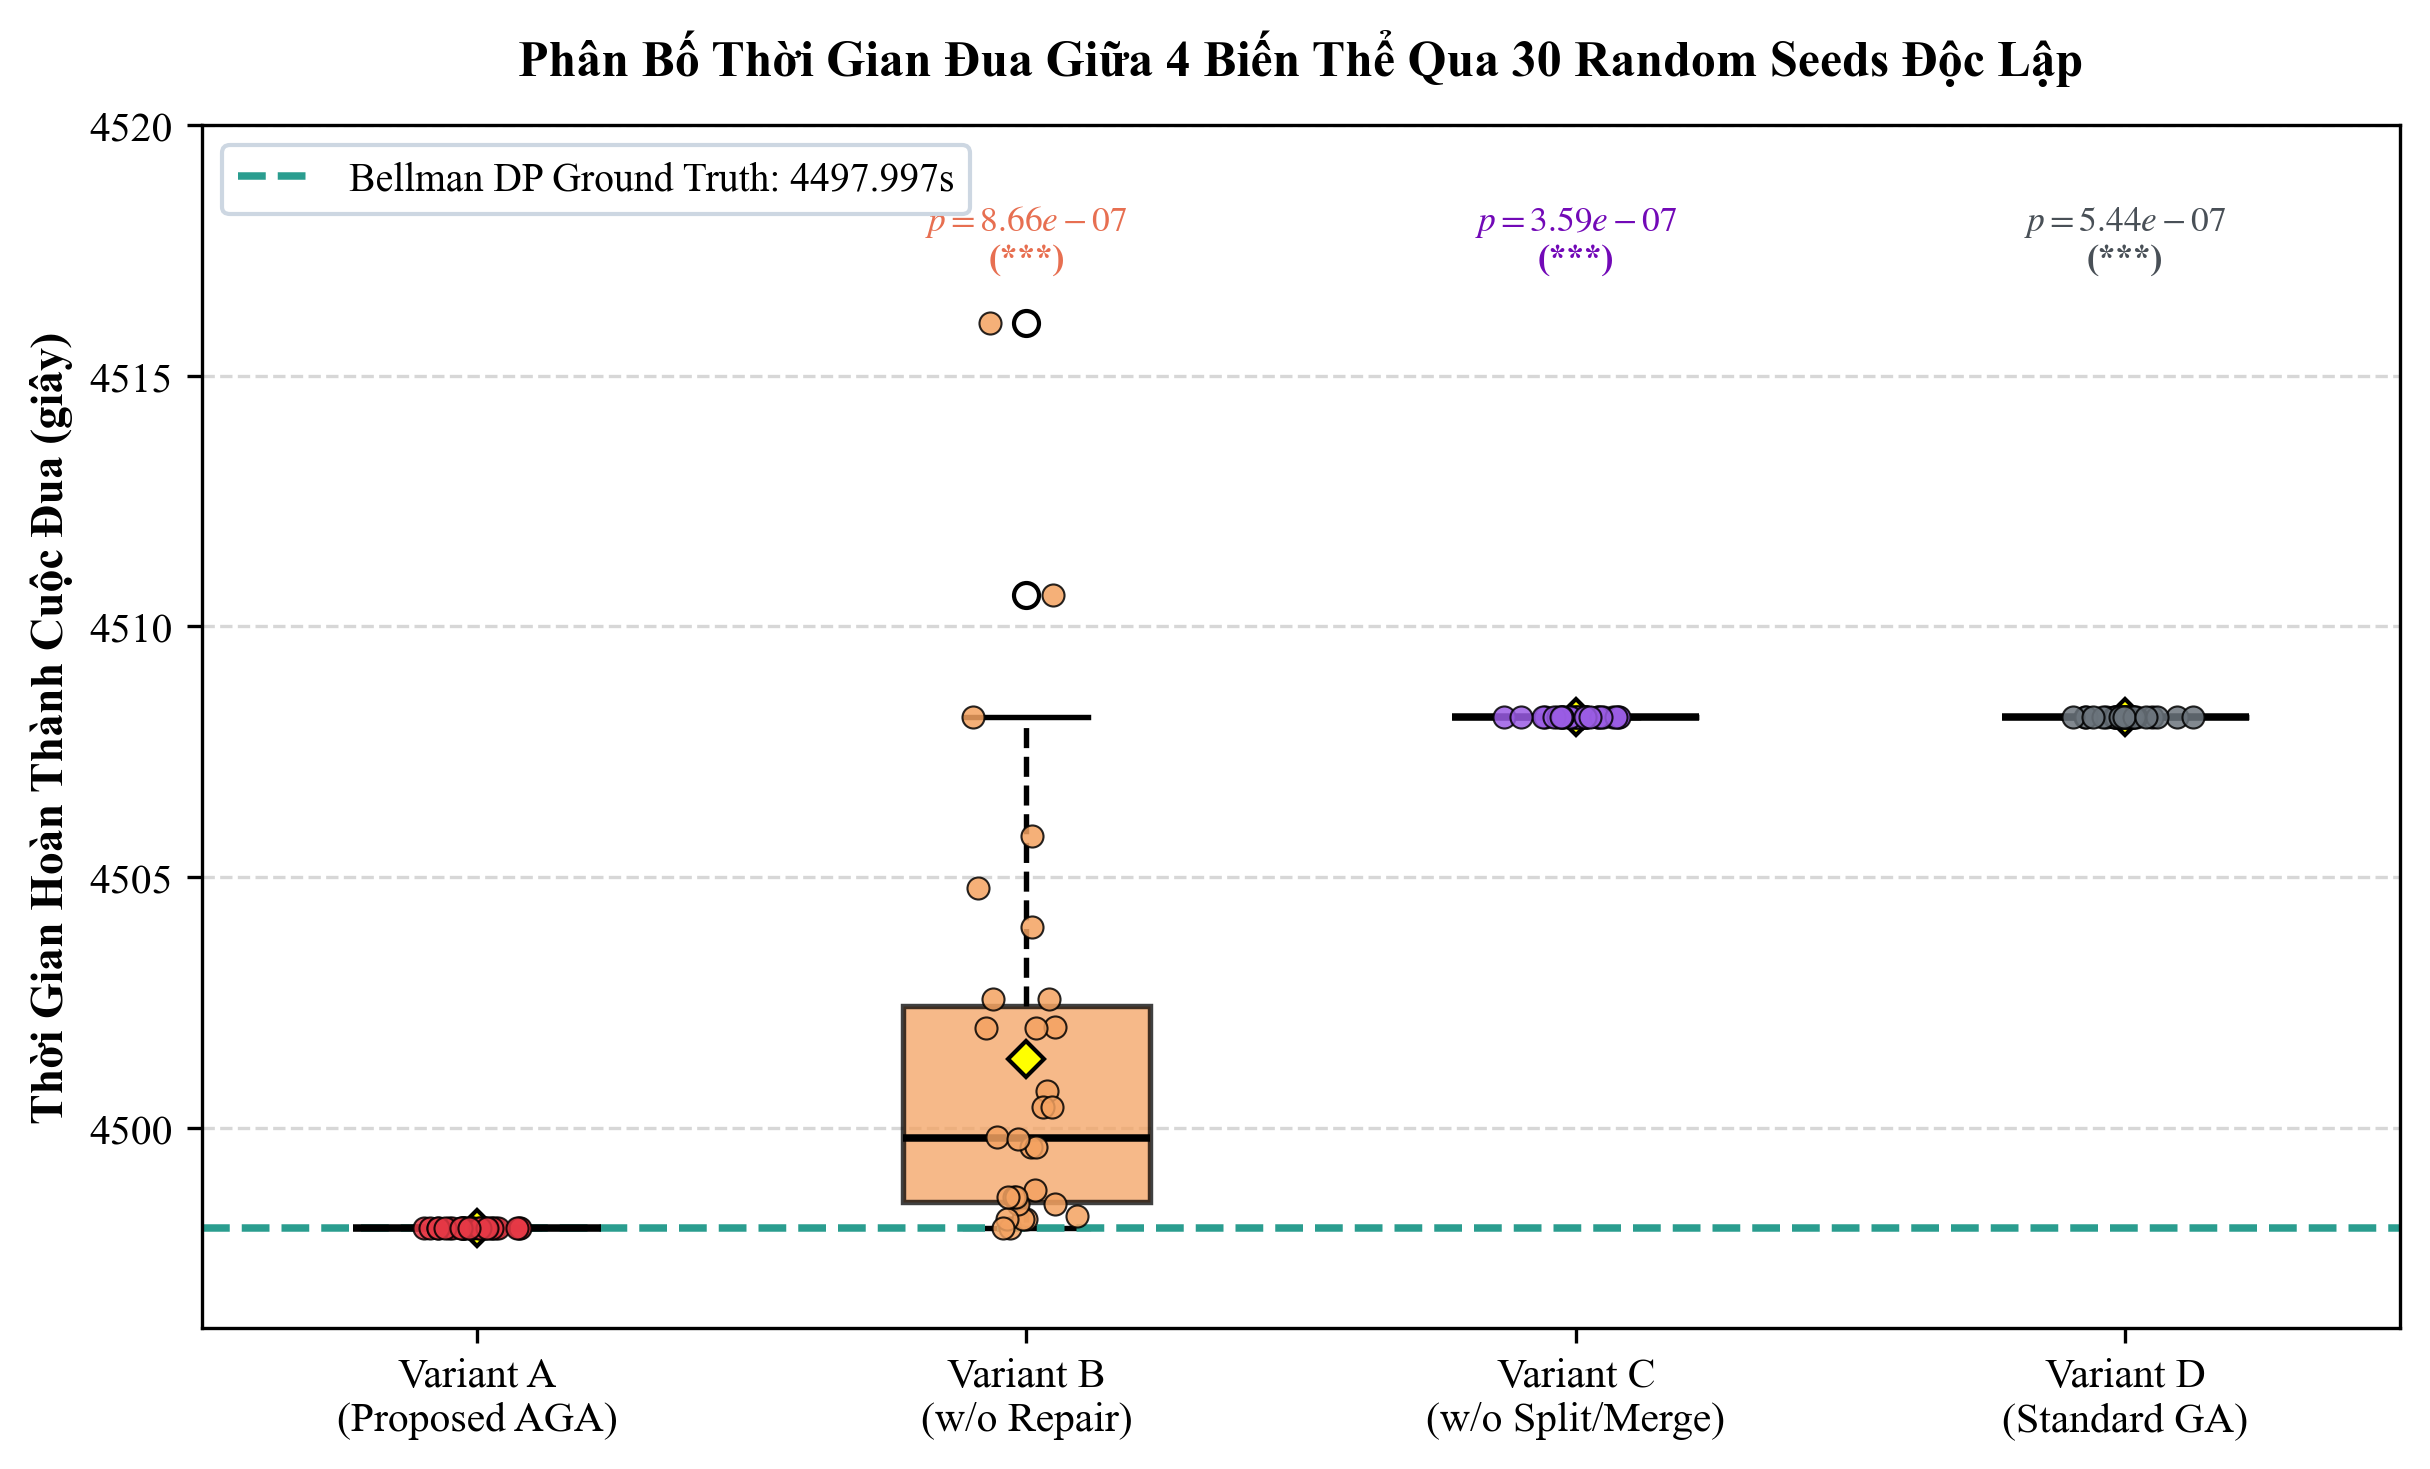
\includegraphics[width=\textwidth,height=0.68\textheight,keepaspectratio]{figures/seed_distribution_boxplot.png}
        \vspace{0.05cm}
        \captionof{figure}{\tiny Biểu đồ Boxplot phân bố thời gian qua 30 random seeds độc lập}
      \end{center}
    \end{column}
  \end{columns}
\end{frame}

% ------------------------------------------------------------------------------
% SLIDE 15: PHÂN TÍCH ĐƯỜNG CONG HỘI TỤ & KIỂM ĐỊNH THỐNG KÊ WILCOXON
% ------------------------------------------------------------------------------
\begin{frame}{14. Phân Tích Đường Cong Hội Tụ \& Kiểm Định Thống Kê}
  \vspace{-0.2cm}
  \begin{columns}[T]
    \begin{column}{0.48\textwidth}
      \begin{center}
        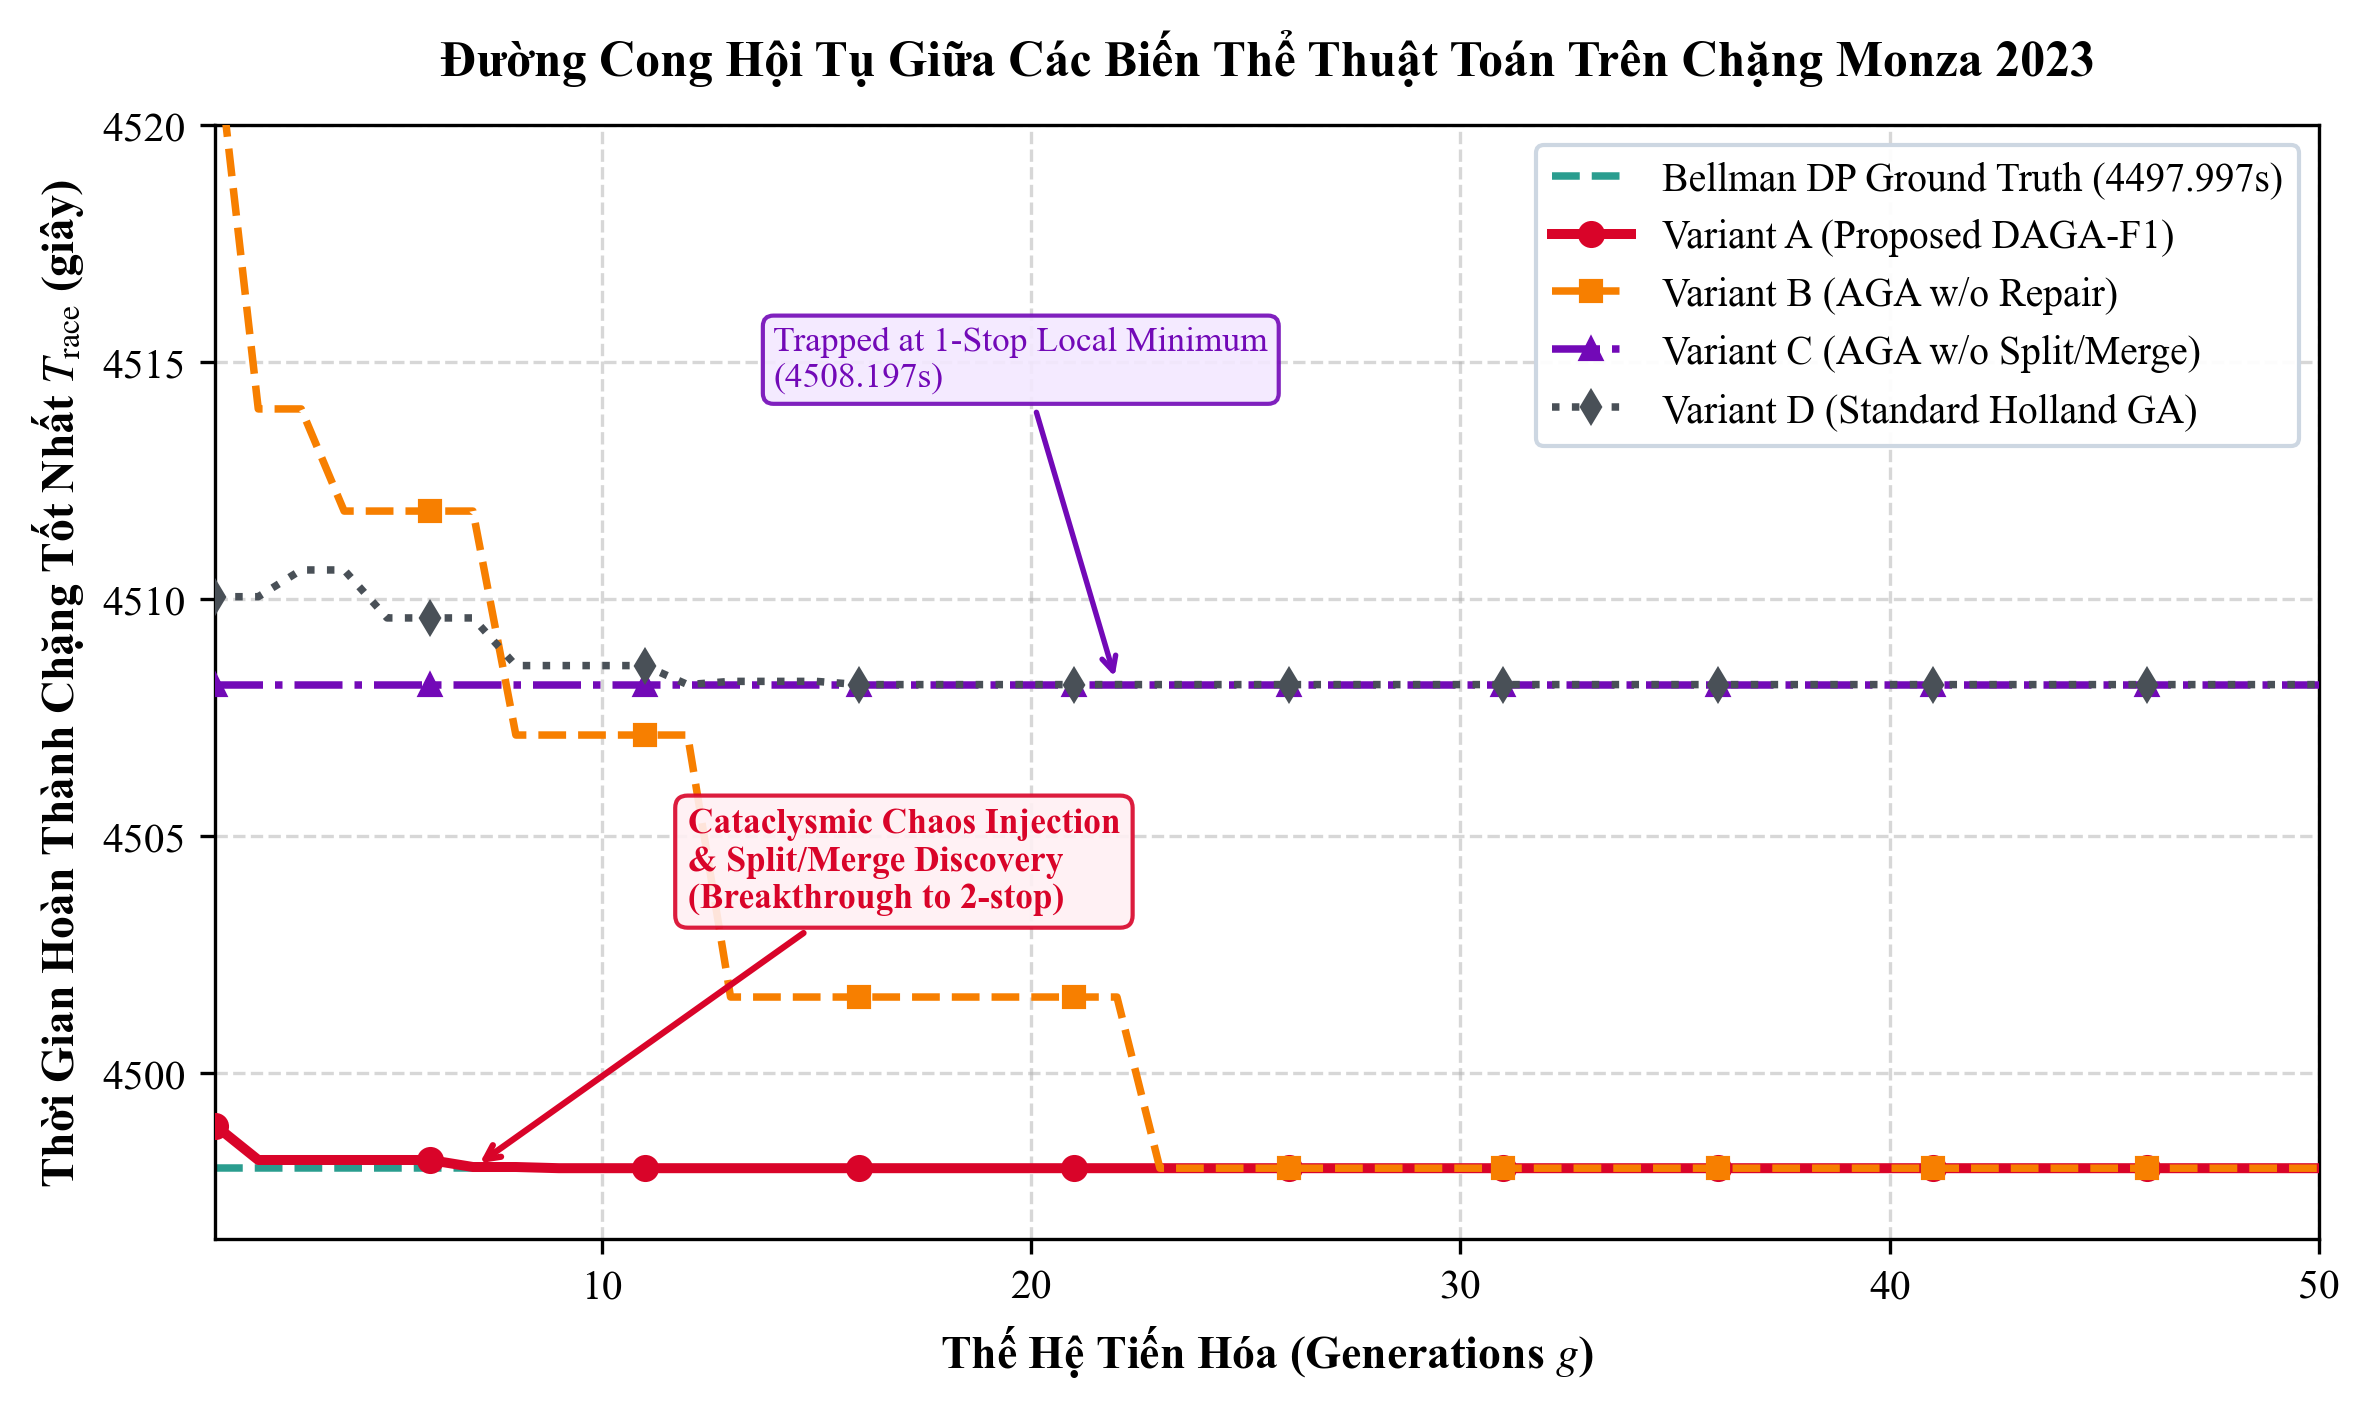
\includegraphics[width=\textwidth,height=0.68\textheight,keepaspectratio]{figures/convergence_comparison.png}
        \vspace{0.05cm}
        \captionof{figure}{\tiny Đường cong hội tụ qua 50 thế hệ: DAGA-F1 bứt phá khỏi hố 1-stop}
      \end{center}
    \end{column}

    \begin{column}{0.50\textwidth}
      \begin{block}{\textbf{3 Phát Hiện Học Thuật Quan Trọng}}
        \small
        \begin{enumerate}
          \item \textbf{Sức mạnh của Split/Merge:} Không có Split/Merge, cả Variant C và Holland GA bị kẹt cứng ở 1-stop ($4508.2\,\text{s}$), chậm hơn chiến lược tối ưu tới \textbf{$10.20\,\text{giây}$}.
          \item \textbf{Sửa nghiệm vật lý giữ 100\% cá thể sống:} Không có Physics Repair (Variant B), $54.6\%$ cá thể chết yểu, độ lệch chuẩn tăng vọt $\sigma = 4.14\,\text{s}$.
        \end{enumerate}
      \end{block}

      \begin{alertblock}{\textbf{Kiểm Định Wilcoxon Signed-Rank Test}}
        \small
        So sánh một phía với DAGA-F1 (Variant A):
        \begin{itemize}
          \item vs Variant B (w/o Repair): $p = 8.66 \times 10^{-7} < 0.001$ (***)
          \item vs Variant C (w/o Split): $p = 3.59 \times 10^{-7} < 0.001$ (***)
          \item vs Standard Holland GA: $p = 5.44 \times 10^{-7} < 0.001$ (***)
        \end{itemize}
        $\implies$ Vượt trội có ý nghĩa thống kê áp đảo tuyệt đối!
      \end{alertblock}
    \end{column}
  \end{columns}
\end{frame}

% ------------------------------------------------------------------------------
% SLIDE 16: KIỂM CHỨNG TỔNG QUÁT HÓA SILVERSTONE GP
% ------------------------------------------------------------------------------
\begin{frame}{15. Kiểm Chứng Tổng Quát Hóa: Silverstone GP (52 Vòng)}
  \begin{columns}[T]
    \begin{column}{0.48\textwidth}
      \begin{block}{\textbf{Thử Thách Khắc Nghiệt Tại Silverstone}}
        \small
        \begin{itemize}
          \item Trường đua tốc độ cao với các góc cua liên hoàn (Maggotts, Becketts, Chapel, Stowe).
          \item Tải trọng khí động học cực đại, độ nhám mặt đường cao $\implies$ Tốc độ mòn lốp nhanh gấp đôi Monza.
          \item Tổn thất làn pit: $T_{\text{pit}} = 20.8\,\text{giây}$.
          \item Ngưỡng an toàn lốp co ngắn: Soft $\le 18$, Med $\le 30$, Hard $\le 42$ vòng.
        \end{itemize}
      \end{block}
    \end{column}

    \begin{column}{0.48\textwidth}
      \begin{exampleblock}{\textbf{Kết Quả Đối Soát Bellman DP vs DAGA-F1}}
        \small
        \begin{itemize}
          \item \textbf{Bellman DP Ground Truth:}
          $$\mathbf{T_{\text{opt}} = 4821.816\,\text{giây}}$$
          Chiến thuật: \badgeMed (19) $\to$ \badgeSoft (14) $\to$ \badgeMed (19)
          \item \textbf{DAGA-F1 Kết Quả:}
          $$\mathbf{T_{\text{AGA}} = 4821.816\,\text{giây}}$$
          Chiến thuật: \badgeSoft (14) $\to$ \badgeMed (19) $\to$ \badgeMed (19)
          \item \textbf{Optimality Gap = 0.0000\%} tuyệt đối!
          \item Runtime: $0.155\,\text{giây}$.
        \end{itemize}
        $\implies$ Khẳng định giải thuật thích ứng tổng quát, hoàn toàn không bị hiện tượng quá khớp (overfitting)!
      \end{exampleblock}
    \end{column}
  \end{columns}
\end{frame}

% ------------------------------------------------------------------------------
% SLIDE 17: HỆ THỐNG KIỂM ĐỊNH CHẤT LƯỢNG 48/48 TESTS & DASHBOARD
% ------------------------------------------------------------------------------
\begin{frame}{16. Hệ Thống Kiểm Định Chất Lượng \& Giao Diện Tương Tác}
  \begin{columns}[T]
    \begin{column}{0.48\textwidth}
      \begin{block}{\textbf{48/48 Unit Tests Tự Động (100\% Pass trong 11.7s)}}
        \small
        Bộ kiểm thử tự động toàn diện kiểm định:
        \begin{itemize}
          \item \textbf{Tính toán giải tích:} Kiểm chứng công thức Faulhaber $O(1)$ sai số $< 10^{-12}$.
          \item \textbf{Sửa nghiệm 10.000 cá thể ngẫu nhiên:} Bảo đảm $100\%$ tuân thủ luật FIA và $\sum l_k = 53$.
          \item \textbf{Kiểm định nhiệt độ mặt đường $T_{\text{track}}$:} Kiểm tra vùng lạnh ($12^\circ\text{C}$ Vegas) đến sa mạc lửa ($62^\circ\text{C}$).
          \item \textbf{Đột biến 2.000 lần liên tục:} Không bao giờ xuất hiện ngoại lệ hoặc crash hệ thống.
        \end{itemize}
      \end{block}
    \end{column}

    \begin{column}{0.48\textwidth}
      \begin{exampleblock}{\textbf{Streamlit Interactive Strategy Dashboard}}
        \small
        \begin{itemize}
          \item \textbf{Giao diện trực quan hóa:} So sánh đồng thời 4 thuật toán trên biểu đồ tương tác đa chiều.
          \item \textbf{Bộ điều khiển thời gian thực:} Tùy chỉnh nhiệt độ mặt đường $T_{\text{track}}$, hệ số mòn, và chi phí pit tức thì.
          \item \textbf{Giả lập Xe An Toàn tương tác:} Chọn vòng xuất hiện Safety Car để quan sát DAGA-F1 tái tối ưu chiến lược trong $5\,\text{ms}$.
          \item Đạt tiêu chuẩn phần mềm khoa học sẵn sàng ứng dụng trên Pit-wall!
        \end{itemize}
      \end{exampleblock}
    \end{column}
  \end{columns}
\end{frame}

% ------------------------------------------------------------------------------
% SLIDE 18: TỔNG KẾT ĐÓNG GÓP & HƯỚNG PHÁT TRIỂN
% ------------------------------------------------------------------------------
\begin{frame}{17. Tổng Kết Đóng Góp \& Hướng Phát Triển Mở Rộng}
  \begin{columns}[T]
    \begin{column}{0.48\textwidth}
      \begin{block}{\textbf{4 Đóng Góp Khoa Học Cốt Lõi Của Đề Án}}
        \small
        \begin{enumerate}
          \item \textbf{Mô hình hóa động lực học lốp bậc hai} kết hợp WLS-Tikhonov-Huber bóc tách viễn trắc FastF1 thực tế.
          \item \textbf{Thước đo Bellman DP 30.088 trạng thái} làm Ground Truth giải tích chuẩn xác tuyệt đối ($4497.997\,\text{s}$).
          \item \textbf{Giải thuật DAGA-F1 với 4 ý tưởng đột phá:} Đạt \textbf{Gap = 0.0000\%}, $100\%$ nghiệm hợp lệ qua 30 random seeds độc lập ($p < 0.001$).
          \item \textbf{Tác chiến Safety Car siêu tốc trong 5 ms}, mở ra khả năng triển khai thực tế trên Pit-wall F1.
        \end{enumerate}
      \end{block}
    \end{column}

    \begin{column}{0.48\textwidth}
      \begin{exampleblock}{\textbf{Hướng Nghiên Cứu Mở Rộng Tiếp Theo}}
        \small
        \begin{itemize}
          \item \textbf{Thời tiết mưa ngẫu nhiên:} Mở rộng mô hình Markov cho điều kiện thời tiết hỗn hợp (chuyển đổi lốp Intermediate / Wet).
          \item \textbf{Lý thuyết trò chơi đa tác tử (Multi-Agent Game Theory):} Dự đoán và phản đòn chiến thuật của đối thủ trên đường đua (Khắc chế Undercut / Overcut).
          \item \textbf{Tích hợp suy biến khí động học (Dirty Air Dynamics):} Mô hình hóa tổn thất lực ép khi chạy bám đuôi đối thủ trong khoảng cách $< 1.0\,\text{giây}$.
        \end{itemize}
      \end{exampleblock}
    \end{column}
  \end{columns}
\end{frame}

% ------------------------------------------------------------------------------
% SLIDE 19: LỜI CẢM ƠN & HỎI ĐÁP
% ------------------------------------------------------------------------------
\begin{frame}[plain]
  \vspace{1.0cm}
  \centering
  \tikz{
    \node[fill=f1navy, text=white, rounded corners=6pt, inner sep=12pt, drop shadow] {
      \Large \textbf{XIN TRÂN TRỌNG CẢM ƠN THẦY VÀ CÁC BẠN ĐÃ LẮNG NGHE!}
    };
  }
  \vspace{0.8cm}
  
  \begin{block}{\centering \textbf{PHIÊN THẢO LUẬN \& GIẢI TRÌNH HỌC THUẬT (Q\&A)}}
    \centering \small
    \vspace{0.1cm}
    \textbf{Nhóm Nghiên Cứu Đề Án DS106 -- Khoa Khoa học Dữ liệu, Trường ĐH Công nghệ Thông tin (UIT)}\\
    \vspace{0.1cm}
    \textit{Mã nguồn, dữ liệu thực nghiệm và tài liệu toán học đã được đồng bộ hóa hoàn chỉnh.}
  \end{block}
\end{frame}

\end{document}
